\documentclass[11pt]{article}
\usepackage[margin=1in]{geometry}
\usepackage{amsmath,amssymb,booktabs,graphicx,setspace,caption,hyperref}
\usepackage[T1]{fontenc}
\usepackage{mathpazo}
\setlength{\parindent}{0pt}
\setlength{\parskip}{0.6em}
\captionsetup{font=small,skip=6pt}
\title{Panel MS-AR(1) with random-effects intercepts, 1970Q1 onward}
\author{}
\date{}
\begin{document}
\maketitle
\section{Model}
Joint panel Markov-switching AR(1) around a \emph{linear} trend, with three regimes:
\begin{align}
y_{it} &= a_i + g\, t + z_{it}, \\
z_{i,t+1} &= \bigl(1-\rho(s_{it})\bigr)\mu(s_{it}) + \rho(s_{it})\, z_{it} + \sigma(s_{it})\,\varepsilon_{it}, \\
s_{i,t+1} &\sim \Pi(\,\cdot\mid s_{it}), \\
a_i &\sim \mathcal{N}(\alpha,\omega^2) \quad \text{(random effects)}.
\end{align}
The trend is linear in calendar time $t$ ($g$ per year, common across countries). In the pooled specification $a_i\equiv a$. In the random-effects specification the $a_i$ are i.i.d.\ Normal draws; $\alpha$ and $\omega$ are estimated by maximum likelihood, integrating each country's Hamilton-filter likelihood by 11-point Gauss--Hermite quadrature. Cycles are plotted using the posterior mean of $a_i$. Latent paths $s_{it}$ are country-specific. The regime dated $t$ governs the transition from $z_t$ to $z_{t+1}$. $\sigma$ and $\rho$ switch with the regime. The median $\mu$ is pinned at 0. $|\rho|<0.995$.
Standard errors (in parentheses) are delta-method from a numerical Hessian on shared parameters. $\pi$ is the ergodic distribution of $\Pi$. $E[z]$ is the long-run mean of the cycle implied by $\mu$, $\rho$, and $\Pi$.
\clearpage
\section{Common intercept and linear trend}
SOE sample from 1970Q1: log real GDP per worker. 62 countries, 6924 observations, 1970-Q1--2024-Q3. Fitted countries: 62. Observations: 6924. Log-likelihood: 16652.31. Ergodic mean of the cycle $E[z]=0.3934$ (0.1970).
Common intercept $a=-3.8544$ (0.1934). Common slope $g=0.0124$ (0.0009).
\begin{table}[h]
\centering
\caption{Regime AR(1), transition matrix, and ergodic $\pi$. Columns are regimes.}
\begin{tabular}{lccc}
\toprule
 & (0) & (1) & (2) \\
\midrule
$\mu$ & -0.6834 & 0.0000 & 1.3119 \\
 & (0.1942) & --- & (0.2051) \\ \addlinespace
$\sigma$ & 0.0109 & 0.1086 & 0.0242 \\
 & (0.0002) & (0.0050) & (0.0004) \\ \addlinespace
$\rho$ & 0.9950 & 0.9950 & 0.9950 \\
 & (0.0000) & (0.0000) & (0.0000) \\ \addlinespace
$\Pi_{0\cdot}$ & 0.9706 & 0.0198 & 0.0096 \\
 & (0.0036) & (0.0035) & (0.0031) \\ \addlinespace
$\Pi_{1\cdot}$ & 0.0714 & 0.7053 & 0.2233 \\
 & (0.0192) & (0.0386) & (0.0376) \\ \addlinespace
$\Pi_{2\cdot}$ & 0.0149 & 0.0206 & 0.9646 \\
 & (0.0032) & (0.0038) & (0.0044) \\ \addlinespace
$\pi$ & 0.4181 & 0.0642 & 0.5177 \\
 & (0.0366) & (0.0085) & (0.0360) \\ \addlinespace
\bottomrule
\end{tabular}
\end{table}
\begin{figure}[h]
\centering
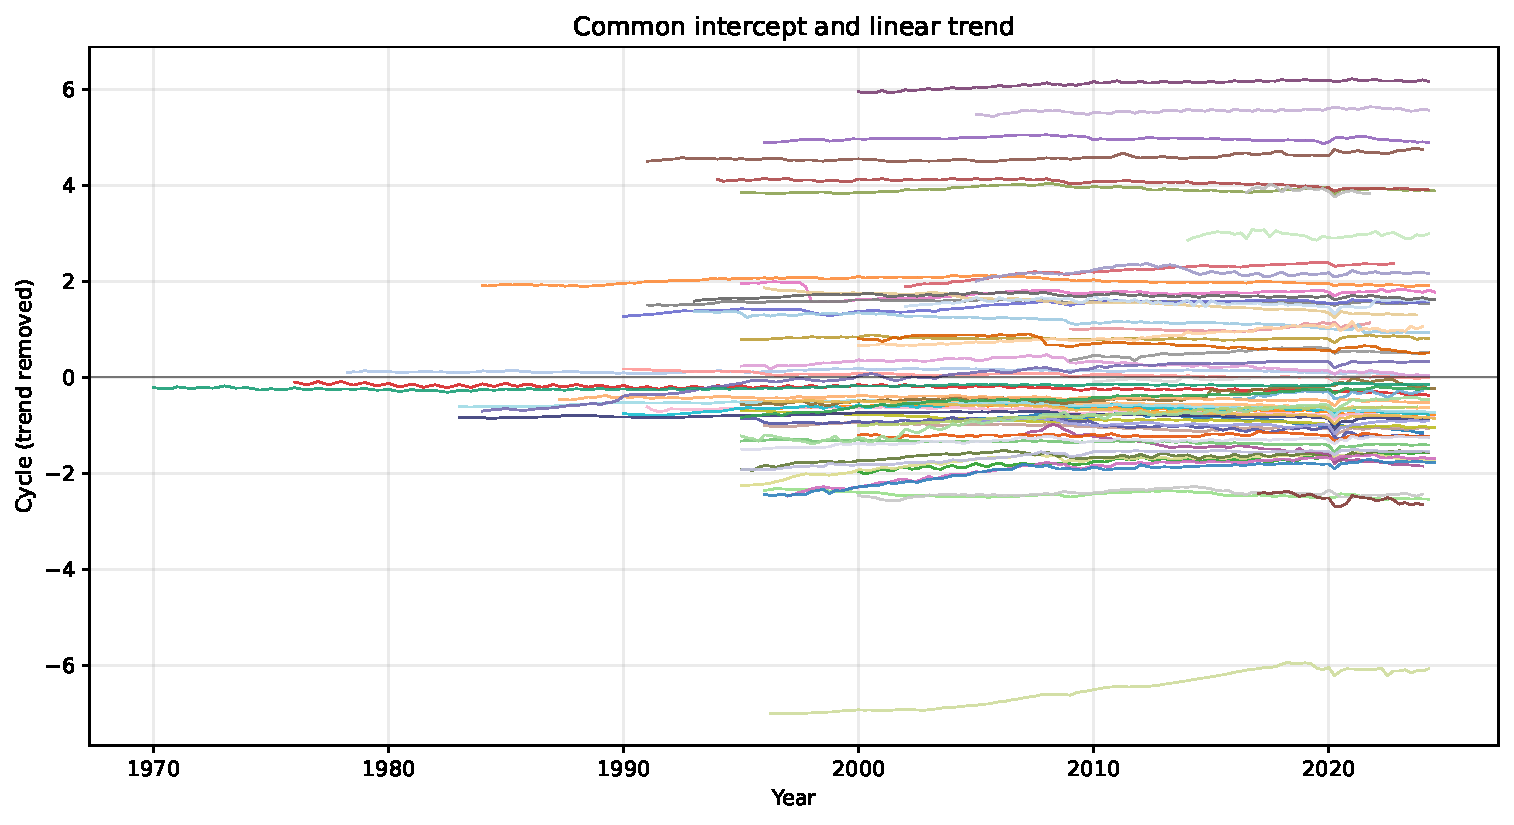
\includegraphics[width=0.75\textwidth]{figs/cycle_re1970_common_ag.pdf}
\caption{Country cycles after removing the linear trend.}
\end{figure}
\clearpage
\section{Random-effects intercepts, common linear trend}
SOE sample from 1970Q1: log real GDP per worker. 62 countries, 6924 observations, 1970-Q1--2024-Q3. Fitted countries: 62. Observations: 6924. Log-likelihood: 17673.12. Ergodic mean of the cycle $E[z]=0.2136$ (0.0460).
Random intercepts $a_i\sim N(\alpha,\omega^2)$ with $\alpha=-3.9761$ (0.0693), $\omega=1.1868$ (0.0133). Posterior-mean $a_i$: mean -3.514, min -8.631, max 2.181. Common slope $g=0.0084$ (0.0007).
\begin{table}[h]
\centering
\caption{Regime AR(1), transition matrix, and ergodic $\pi$. Columns are regimes.}
\begin{tabular}{lccc}
\toprule
 & (0) & (1) & (2) \\
\midrule
$\mu$ & -0.5933 & 0.0000 & 0.5486 \\
 & (0.2441) & --- & (0.0620) \\ \addlinespace
$\sigma$ & 0.0680 & 0.0220 & 0.0097 \\
 & (0.0031) & (0.0006) & (0.0002) \\ \addlinespace
$\rho$ & 0.9950 & 0.9950 & 0.9950 \\
 & (0.0000) & (0.0000) & (0.0000) \\ \addlinespace
$\Pi_{0\cdot}$ & 0.7820 & 0.1448 & 0.0732 \\
 & (0.0317) & (0.0299) & (0.0177) \\ \addlinespace
$\Pi_{1\cdot}$ & 0.0201 & 0.9581 & 0.0218 \\
 & (0.0046) & (0.0060) & (0.0045) \\ \addlinespace
$\Pi_{2\cdot}$ & 0.0202 & 0.0124 & 0.9673 \\
 & (0.0035) & (0.0039) & (0.0038) \\ \addlinespace
$\pi$ & 0.0847 & 0.4352 & 0.4801 \\
 & (0.0121) & (0.0337) & (0.0346) \\ \addlinespace
\bottomrule
\end{tabular}
\end{table}
\begin{figure}[h]
\centering
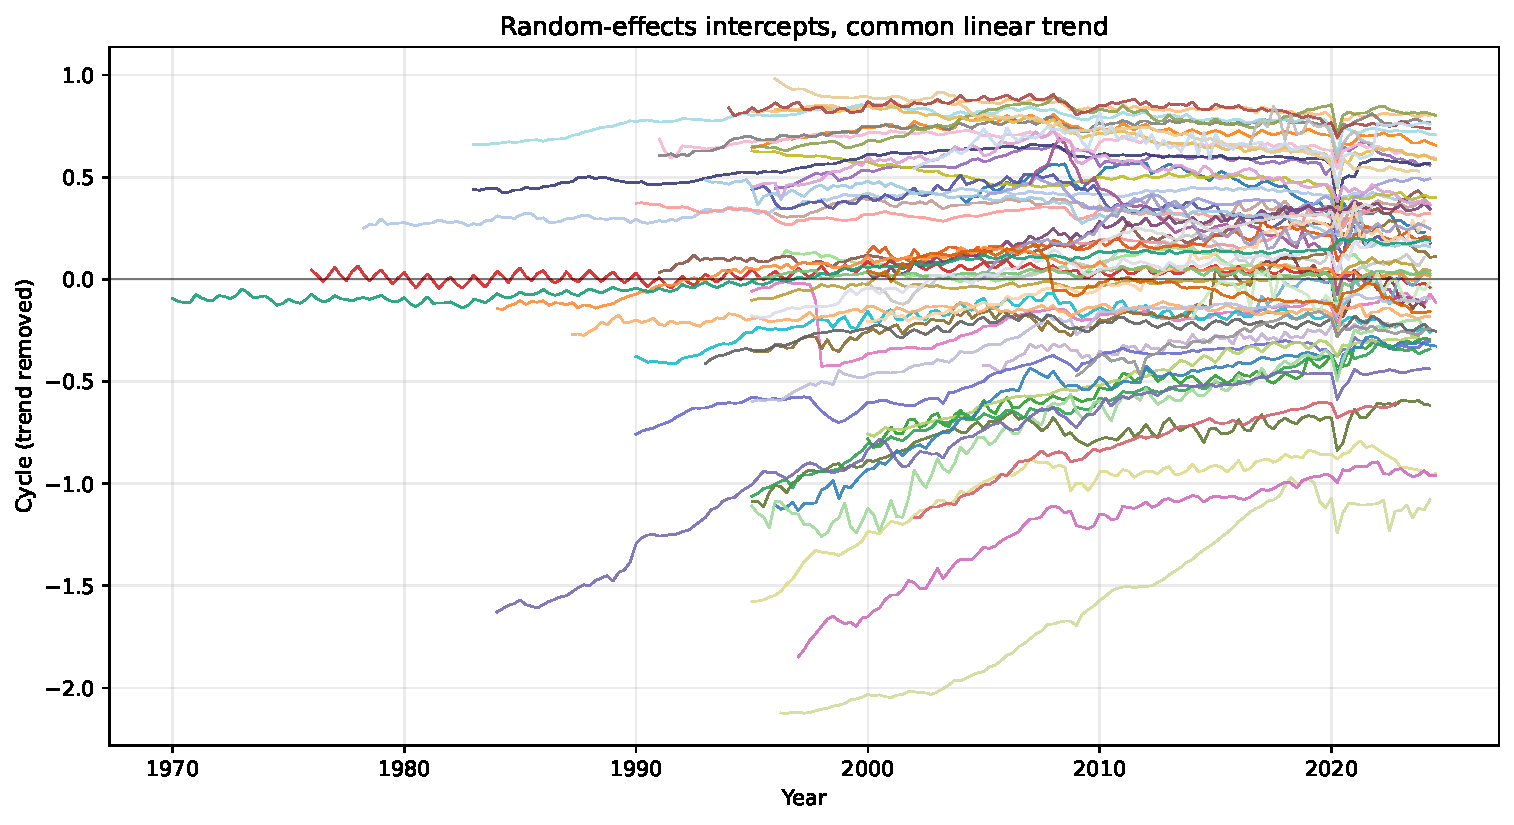
\includegraphics[width=0.75\textwidth]{figs/cycle_re1970_re_ai.pdf}
\caption{Country cycles after removing the linear trend.}
\end{figure}
\end{document}
